\newpage
\section{Diagramme de cas d'utilisation}

Le diagramme de cas d'utilisation (figure \ref{useCase}) essaie de présenter les différentes actions réalisables grâce à notre application. Toute action nécessite d'abord de s'être identifié.

\begin{figure}[h!]
  \centering
  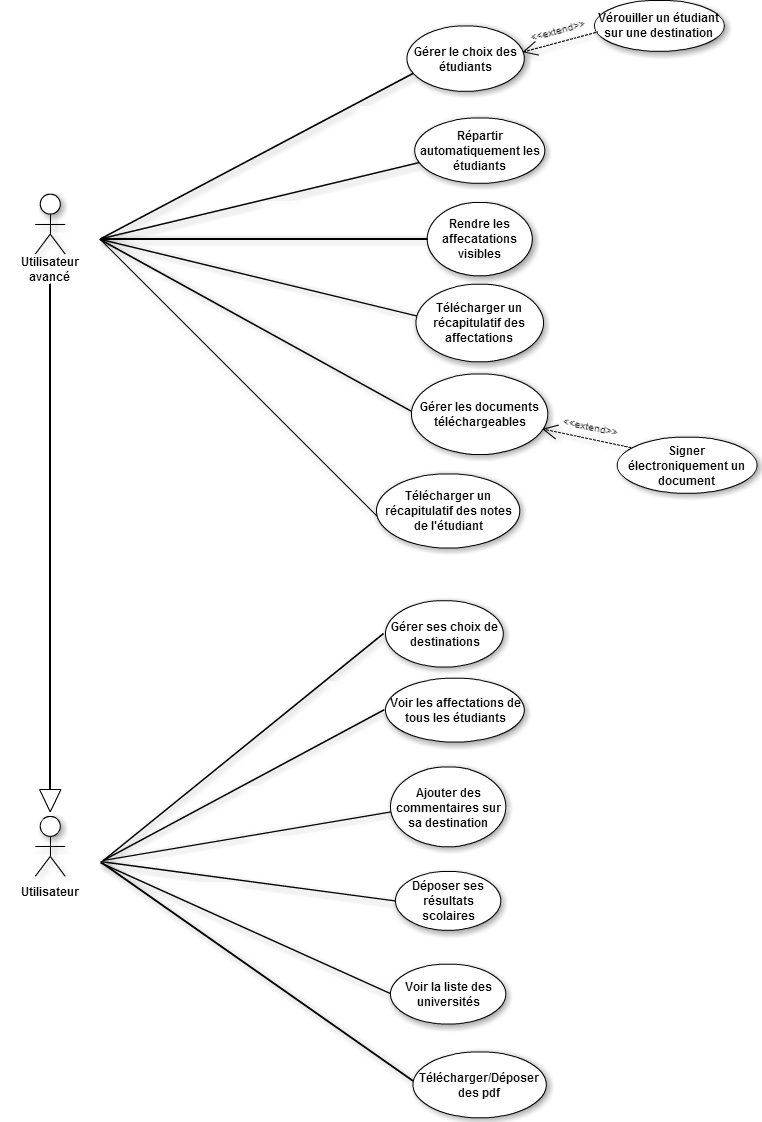
\includegraphics[scale=0.4]{Projet/useCaseDiag/useCaseDiagram.png}
  \caption{Diagramme de cas d'utilisation}
  \label{useCase}
\end{figure}

